\chapter{Optimised Loading of Change-based Persistence}
This paper proposes and evaluates an efficient approach for loading models stored in a change-based format. The work builds on language-independent change-based persistence (CBP) of models conforming to object-oriented metamodelling architectures such as MOF and EMF, an approach which persists a model's editing history rather than its current state. We evaluate the performance of the proposed loading approach and assess its impact on saving change-based models. Our results show that the proposed approach significantly improves loading times compared to the baseline CBP loading approach, and has a negligible impact on saving.

\section{Introduction}
\label{sec:introduction}
Conventional approaches for file-based model persistence in metamodelling architectures such as MOF \cite{omg2018mof} and EMF \cite{steinberg2008emf} are state-based -- saving the current state of a model.  In these approaches,  version control and change detection are delegated to external systems.  State-based persistence is computationally expensive, as a whole model must be saved and loaded; this can particularly affect large models and collaborative developments.

In \cite{yohannis2017turning}, we proposed change-based persistence (CBP), an approach that persists the full sequence of \emph{changes} made to a model instead of persisting the state. Compared to state-based approaches, CBP supports fast detection of changes, which can speed up model comparison and merging, as well as fast incremental model validation and transformation \cite{rath2012derived,ogunyomi2015property}. However, saving the change history of a model results in large, and ever-growing, CBP files.  Loading times are also significant, as the loading process has to reconstruct a model's current state from its history \cite{yohannis2017turning}.   This paper proposes and evaluates an approach that reduces CBP model loading time by avoiding the replaying of historical changes that have no impact on the final state of the model.

The rest of the paper is structured as follows. Section \ref{sec:case_study} introduces a running example and provides a brief introduction to CBP.
Section \ref{sec:loading_time_optimisation} presents the approach to speed up model loading and its supporting data structures. Section \ref{sec:performance_evaluation} presents experimental results and evaluation. Section \ref{sec:related_work} provides an overview of related work, and Section \ref{sec:conclusions} concludes with a discussion on directions of future work.

\vspace{-15pt}
\section{Running Example}
\label{sec:case_study}
\vspace{-10pt}
To explain model CBP, we use a minimal tree metamodel and an example tree model in Fig. \ref{fig:tree_metamodel} and \ref{fig:initial_model}.
The metamodel is expressed in the Eclipse Modelling Framework (EMF) Ecore metamodelling language, the de-facto standard for object-oriented metamodelling.  The example is contrived to avoid unnecessary repetition, whilst providing adequate coverage of the core features of Ecore (classes, single/multi-valued features, references).
In this example, a tree model consists of named nodes which can -- optionally -- contain other nodes ($child$ reference).

\vspace{-20pt}
\begin{figure}[ht]
\begin{subfigure}[t]{0.3\linewidth}
\centering
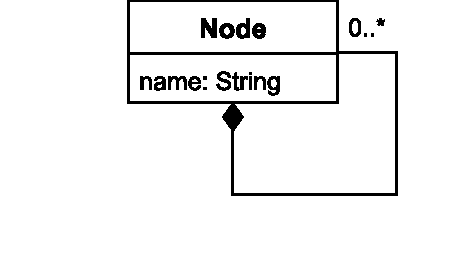
\includegraphics[width=0.8\linewidth]{node_metamodel}
\caption{The tree metamodel (EMF/Ecore).}
\label{fig:tree_metamodel}
\end{subfigure}
\hfill
\begin{subfigure}[t]{0.7\linewidth}
\centering
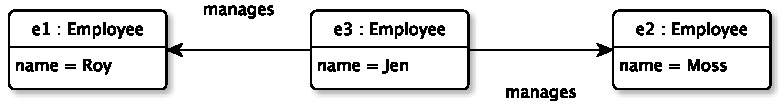
\includegraphics[width=0.6\linewidth]{initial_chart}
\caption{A tree model that conforms to the  metamodel.  Node n3 is created and then deleted.}
\label{fig:initial_model}
\end{subfigure}
\caption{Running example of a metamodel and a conformant model.}
\label{fig:append_speed}
\end{figure}

\vspace{-10pt}
The current state of the model in Fig. \ref{fig:initial_model} has two nodes, $n1$, $n2$.  The model was constructed by firstly creating the three nodes ($n1$, $n2$ and $n3$) and then nodes $n2$ and $n3$ were then added as children of $n1$. Finally, node $n3$ was deleted.

\vspace{-10pt}
\begin{minipage}[t]{0.5\linewidth}
\begin{lstlisting}[style=xmi,caption={State-based tree model.},label=lst:xmimodel]
<Node id="n1" name="A">
<children id="n2" name="B"/>
</Node>
\end{lstlisting}
\end{minipage}
\hfill
\begin{minipage}[t]{0.5\linewidth}
\begin{lstlisting}[style=eol,caption={Change-based tree model.},label=lst:cbpmodel]
create n1 of Node
set n1.name to "A"  
create n2 of Node
set n2.name to "B"  
create n3 of Node
set n3.name to "C"  
add n2 to n1.children   
add n3 to n1.children
remove n3 from n1.children   
delete n3
\end{lstlisting}
\end{minipage}

Listings \ref{lst:xmimodel} shows the state-based representation of the model, using simplified XMI.  Listing \ref{lst:cbpmodel} shows the change-based representation, using the CBP syntax introduced in \cite{yohannis2017turning}. Lines 1-6 of Listing \ref{lst:cbpmodel} record the creation and naming of the three nodes; lines 7-8 record the addition of $n2$ and $n3$ as children of $n1$; lines 9-10 capture the deletion of $n3$ (the $remove$ command removes f $n3$ from its container; the $delete$ command completely removes $n3$ from its model). Changes in a CBP representation can be uniquely identified by their line numbers.

The example model history illustrates a case where  earlier events (creating \emph{n3} in line 5, naming it in line 6, making it a child of \emph{n1} in line 8, removing it from the container in line 9) are superseded by a subsequent event (deletion of \emph{n3} in line 10).  Loading of the current model would arguably be faster if the events in lines 5, 6, 8, 9 and 10 could be ignored.

\vspace{-10pt}
\section{Towards Efficient Loading of Change-Based Models}
\label{sec:loading_time_optimisation}

\vspace{-10pt}
The flowchart in Fig. \ref{fig:flowchart} provides an overview of the editing lifecycle of a CBP model \cite{yohannis2017turning}, with the proposed extensions shown as starred blocks. A model is loaded (1), edited (2) and saved (3).  During editing, the changes made to the model are recorded in a memory-based data structure, serialised and with the latest events appended at the end (4). The change events are persisted into a CBP file every time the model is saved (5). When a model is re-loaded, the current model state is recreated by replaying the events stored in the CBP file (6).

\vspace{-10pt}
\begin{figure}[ht]
\centering
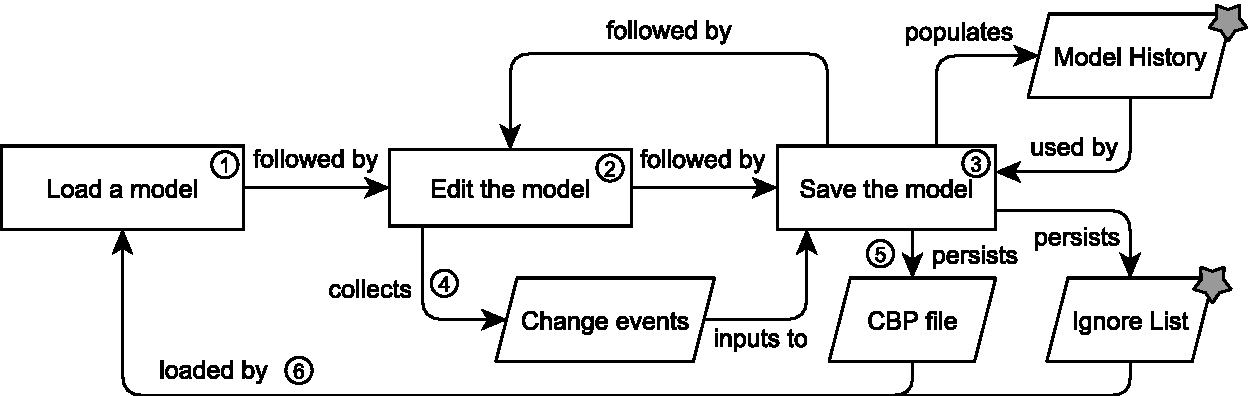
\includegraphics[width=\linewidth]{flowchart}
\caption{CBP workflow, with optimised loading elements indicated by starred blocks.}
\label{fig:flowchart}
\end{figure}

\vspace{-10pt}
A key principle of CBP is that the editing history is immutable, as this is essential for supporting incremental model management operations. As such, superseded events cannot be simply removed from the CBP file. Therefore, the proposed approach adds two artefacts: a in-memory $Model History$ data structure which aggregates change events per model element, and an $Ignore List$ file, which persists the position (i.e. line numbers) of superseded events so that the events can be ignored the next time the model is loaded. The Ignore List is saved alongside the CBP file. The rest of this section presents how the Model History is used to detect superseded events and generate the Ignore List.

\vspace{-10pt}
\subsection{Model History}
\label{subsec:model_history}
The Model History data structure stores events and their line numbers in a CBP representation.  The data can be used to reason about the events of a particular element and to determine which events are superseded.  We refer to the line number in the CBP representation as the \emph{event number}. The proposed data structure is defined in Fig. \ref{fig:object_history} using a class diagram.  

A \emph{ModelHistory} has a \emph{URI} attribute to identify the model for which it records changes.  A \emph{ModelHistory} can link to many \emph{ElementHistory} objects, each identified by its \emph{element} field which is queried from the model. An \emph{ElementHistory} can link to many \emph{FeatureHistories}, representing the editing histories of individual features -- either references or attributes of the element. A \emph{FeatureHistory} has a \emph{type} (attribute or reference) and a \emph{name}, identifying the feature.

\vspace{-20pt}    
\begin{figure}[ht]
\centering
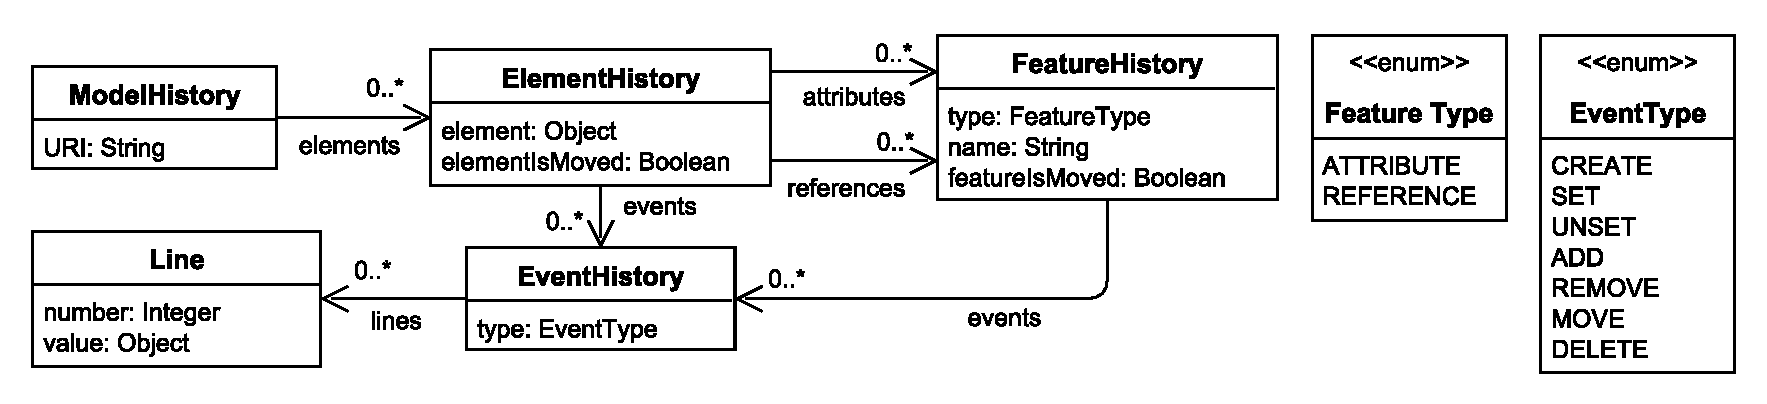
\includegraphics[width=\linewidth]{object_history}
\caption{The class model defining Model History.}
\label{fig:object_history}
\end{figure}

\vspace{-30pt}
\begin{figure}[ht]
\centering
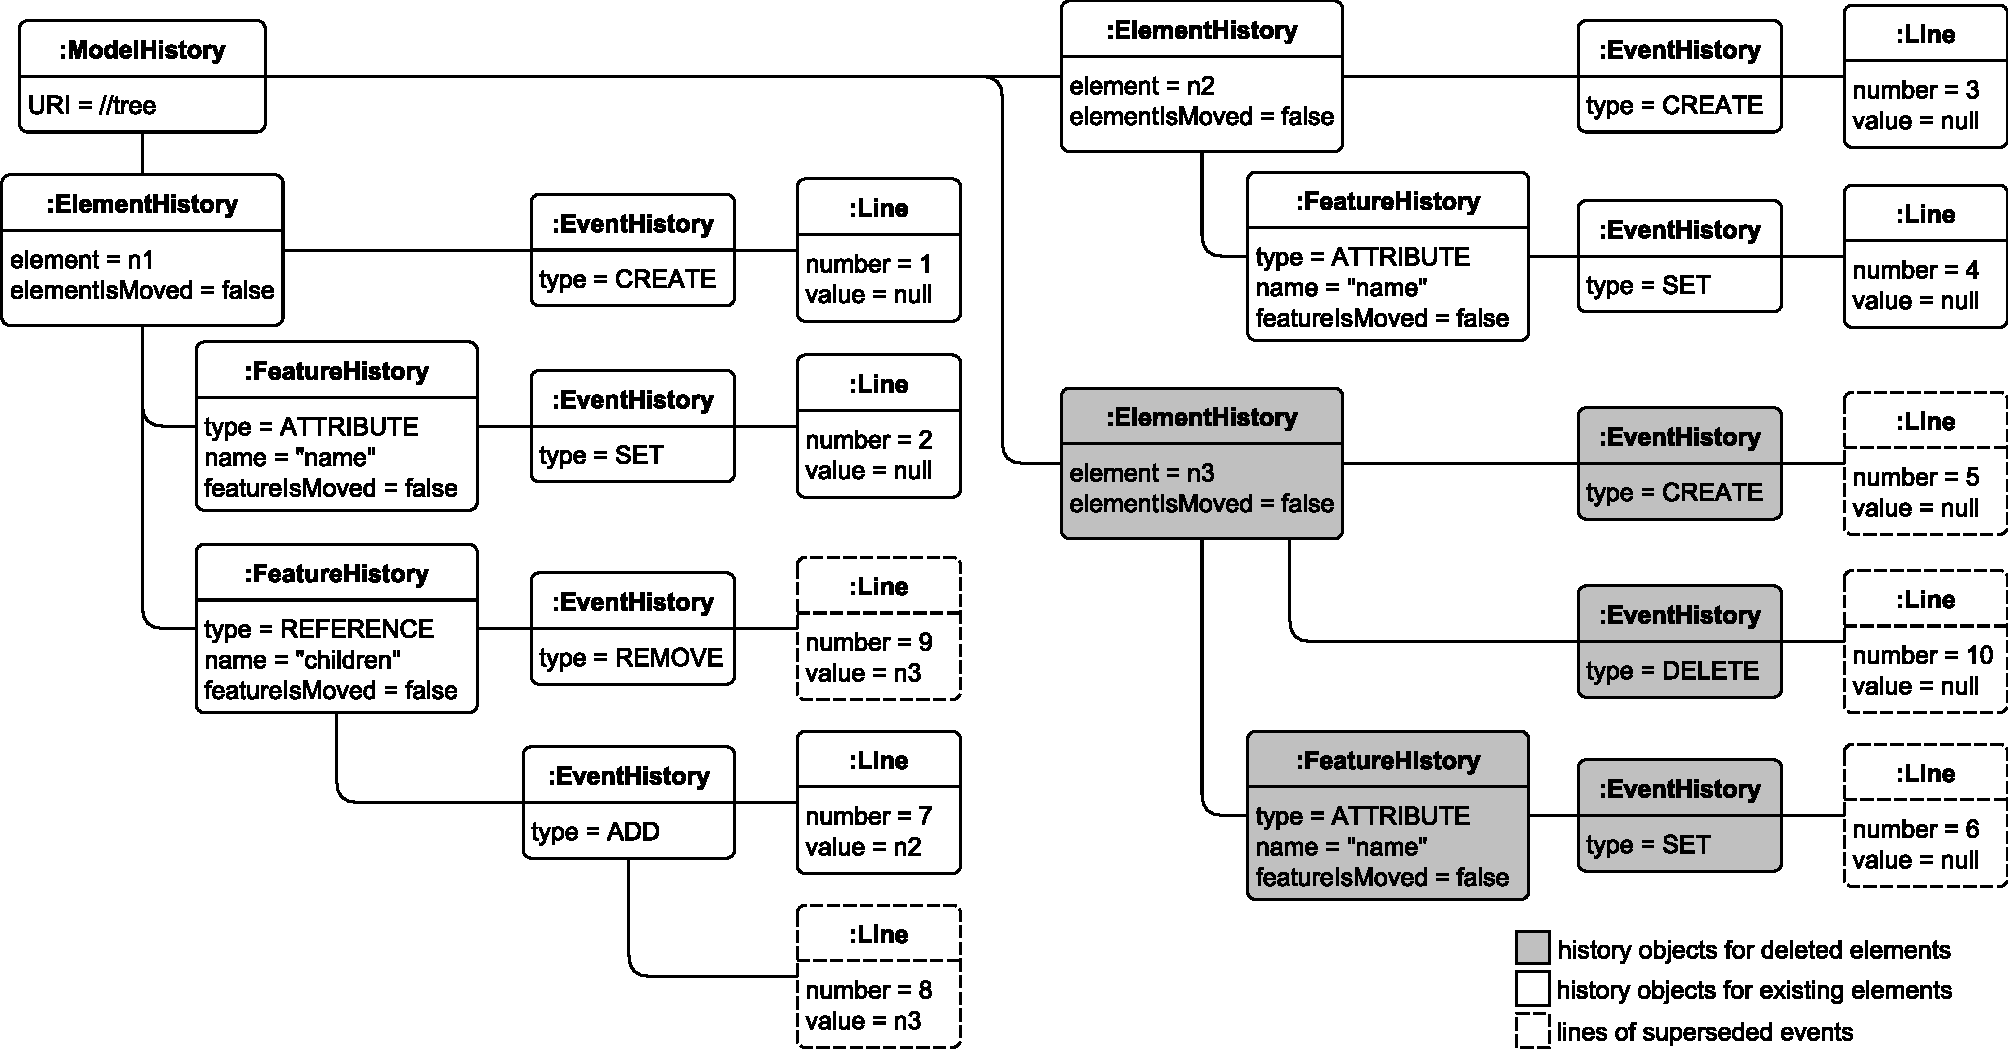
\includegraphics[width=\linewidth]{history_structure}
\caption{The object diagram of the CBP model history in Listing \ref{lst:cbpmodel}.}
\label{fig:history_structure}
\end{figure}

An \emph{EventHistory} represents series of events of the same type; it has an attribute \emph{type} to identify the events' type and can have many \emph{Line}s. A \emph{Line} has a \emph{number} attribute, to record the event number and a \emph{value} that records the element involved in the event (Value is only used for events with types \emph{$ADD$}, \emph{$REMOVE$} and \emph{$MOVE$}). Each \emph{FeatureHistory} can have many \emph{EventHistories}, to represent the events that modify the values of the features. Each \emph{ElementHistory} can have many \emph{EventHistories} to represent events that affect the state of the elements (life-cycle and relations to multivalued features). Fig. \ref{fig:history_structure} shows an object diagram corresponding to the model in Fig. \ref{fig:object_history} that captures the model history shown in Listing \ref{lst:cbpmodel}. The grey rectangles are \emph{History} objects related to the deleted node \emph{n3}. The rectangles with the dashed outline are \emph{Line} objects that represent superseded changes. 

Next, we present the different strategies used to identify superseded events that will be added to the Ignore List.   

\vspace{-10pt}
\subsection{Set and Unset Events}
\label{subsec:set_and_unset_operations}
During the lifecycle of a model, a single-valued feature can have its value set (assigned) or unset many times. Each event is persisted, but only the last assigned value needs to be considered. For example, in Listing \ref{lst:set_unset_example_1}, the feature \emph{name} is set to the value ``A'', unset, and finally set to the value ``B''.  In the final state of the model, \emph{n1.name} = ``B''. Thus, only line 4 is significant for the model's final state and therefore lines 2 and 3 can be ignored when loading the model. For a $set$ event, all preceding $set$ and $unset$ events can be ignored, but for an $unset$ event, all $set$ and $unset$ events can be ignored. Executing it does not have any effect on the final state of a model if all the preceding events also have been ignored.

\vspace{-10pt}
\begin{minipage}[t]{0.49\linewidth}
\begin{lstlisting}[style=eol,caption={A CBP representation of attribute \emph{name} assignments ended with SET.},label=lst:set_unset_example_1]
create n1 of Node
set n1.name to "A"
unset n1.name
set n1.name to "B"
\end{lstlisting}
\end{minipage}
\hfill
\begin{minipage}[t]{0.49\linewidth}
\begin{lstlisting}[style=eol,caption={A CBP representation of attribute \emph{name} assignments ended with UNSET.},label=lst:set_unset_example_2]
create n1 of Node
set n1.name to "A"
set n1.name to "B"
unset n1.name
\end{lstlisting}
\end{minipage}

Based on the Listing \ref{lst:set_unset_example_1}, our approach creates an instance of $ElementHistory$ $n1$ which contains an instance of $FeatureHistory$ $name$. The $FeatureHistory$ $name$ consists of two $EventHistory$ instances, with types $SET$ and $UNSET$ (the instances are named $set$ and $unset$ respectively for brevity). The $set$ records the $Line$ instances that hold the event numbers where the $set$ events, and similarly for $unset$.

From Listing \ref{lst:set_unset_example_1}, we can thus infer that $name$.$set$.$lines$ = $\{2,4\}$ and $name$.$unset$. $lines$ = $\{3\}$. The event numbers in both lists are used to determine that the events represented by lines 2 and 3 are superseded by that in line 4, which is a $set$ event, giving an $ignoreList$ = $\{2, 3\}$.  By the same process, for Listing \ref{lst:set_unset_example_2}, we can reason that $name$.$set$.$lines$ = \{2,3\} and $name$.$unset$.$lines$ = \{4\}.  However, this case, the highest-numbered event is an $unset$, all so line numbers are put into the $ignoreList$ ($ignoreList$ = $\{2, 3, 4\}$) ($unset$ event can be ignored along with all preceding {$set$ and $unset$ events). 

\vspace{-10pt}
\subsection{Add, Remove, and Move Events}\label{subsec:add_remove_and_move_operations}
For a multi-valued feature, add, remove, and move events can be called many times, to modify the feature. If an element is added to the feature, moved multiple times, and finally removed, then all the element's preceding events can be ignored, as long as the order of the feature's elements is not changed. 



Listing \ref{lst:add_move_reference} shows an example without a $move$ event. In the Listing, nodes $n1$, $n2$, and $n3$ are added to the $children$ feature of $p$ (lines 5-7), In the latest state of the model, $children$ only contains $n1$ and $n3$. As a result, the loading process could ignore the events that represent the \textit{$add$} and \textit{$remove$} events on $n1$. 

\vspace{-20pt}
\begin{minipage}[t]{0.34\linewidth}
\begin{lstlisting}[style=eol,caption={A CBP of add and remove operations.},label=lst:add_move_reference]
create p of Node
create n1 of Node
create n2 of Node
create n3 of Node
add n1 to p.children
add n2 to p.children
add n3 to p.children
remove n2 from p.children   
\end{lstlisting}
\end{minipage}
\hfill
\begin{minipage}[t]{0.62\linewidth}
\begin{lstlisting}[style=eol,caption={A CBP representation of add, move, and remove operations.},label=lst:add_remove_move_reference]
create p of Node          //children=[]
create n1 of Node         //children=[]
create n2 of Node         //children=[]
create n3 of Node         //children=[]
add n1 to p.children      //children=[n1]
add n2 to p.children      //children=[n1,n2]
add n3 to p.children      //children=[n1,n2,n3]
move 0 to 1 in p.children //children=[n2,n1,n3]
remove n2 from p.children //children=[n1,n3]
\end{lstlisting}
\end{minipage}

To create the Ignore List for the Listing \ref{lst:add_move_reference}, we can deduce that $children$.$add$. $lines$ = \{\{5, $n1$\}, \{6, $n2$\} \{7, $n3$\}\} (5 is the line number and $n1$ is the value) and $children$.$remove$.$lines$ = \{\{8, $n1$\}\}. Since $n2$ is removed from its containing feature (line 8), then executing its preceding add and remove events is unnecessary. Note that we retain the $create$ event (line 3) as $n2$ has not been deleted from the model -- only removed from its containing feature. We can iterate through the add and move structures to identify the events on $n2$ that should be removed, resulting in the $ignoreList$ = \{6, 8\}.

Listing \ref{lst:add_remove_move_reference} shows an example with a $move$ event\footnote{The commented parts  show the end states of $children$ after each event}. A $move$ event is inserted at line 8 thus makes the $remove$ event of $n2$  moves to line 9. With the introduction of this $move$ event, we now have the $children$.$add$.$lines$ = \{\{5, $n1$\}, \{6, $n2$\} \{7, $n3$\}\}, $children$.$move$.$lines$ = \{\{8, $n1$\}\}, and $children$.$remove$.$lines$ = \{\{9, $n2$\}\}. In the final state of the model, the $children$ should have the $n1$ and $n3$ in order, $children$ = [n1, n3].  

However, executing the previous strategy naively leads to an erroneous final state. Using $ignoreList$ = \{6, 8\} produced by the naive strategy leads to a different order of $n1$ and $n3$ in the final state of the model where $children$ = [n3, n1] as shown by the naive optimised CBP in Listing \ref{lst:naive_add_remove_move_reference}. To overcome this problem, *$IsMoved$ flags in Fig. \ref{fig:object_history} is used to sign  features and elements if they have been moved -- the flags are set to $true$. If an element's *$IsMoved$ flag is true then all of its line numbers related to $add$, $move$, $remove$ events cannot be put into the $ignoreList$. The flags are set to $false$ if the feature is empty. 

\begin{lstlisting}[style=eol,caption={A naive optimised CBP representation of original CBP representation in Listing \ref{lst:add_remove_move_reference} .},label=lst:naive_add_remove_move_reference]
create p of Node            // children = []
create n1 of Node           // children = []
create n2 of Node           // children = []
create n3 of Node           // children = []
add n1 to p.children        // children = [n1]
add n3 to p.children        // children = [n1, n3]
move 0 to 1 in p.children   // children = [n3, n1]
\end{lstlisting}

\subsection{Create and Delete Events}
\label{subsec:create_and_delete_operations}

When an element is deleted, it is completely removed from the model. Therefore, all previous events ($create$, $set$, $unset$, $move$, $add$, $remove$, $delete$) on features of element can be ignored, along with all events on the element's features. For example, when node \emph{n3} in Listing \ref{lst:cbpmodel} is deleted, the events in lines 5-6 and 8-10 are superseded. If the Listing \ref{lst:cbpmodel} is optimised -- some of its events are ignored -- when loading, it runs as if the Listing \ref{lst:cbpmodel_optimised} are executed.

\begin{lstlisting}[style=eol,caption={Change-based representation of the model in Fig. \ref{fig:initial_model} after removal of node $n3$.},label=lst:cbpmodel_optimised]
create n1 of Node
set n1.name to "A"
create n2 of Node
set n2.name to "B"
add n2 to n1.children
\end{lstlisting}

Using the Listing \ref{lst:cbpmodel}, we can construct the structure of histories that are related to element $n3$ as follows: $n3$.$create$.$lines$ = \{5\}, $n3$.$name$.$set$.$lines$ = \{6\}, $n1$.$children$.$add$.$lines$ = \{\{7, $n2$\}, \{8, $n3$\}\}, $n1$.$children$.$remove$.$lines$ = \{\{9, $n3$\}\}, and $n3$.$delete$.$lines$ = \{10\}. Thus, when element $n3$ is deleted, by iterating through all these history structures, all line numbers associated with $n3$ can be identified and added to $ignoreList$ producing $ignoreList$ = \{5 6, 8, 9, 10\} so they can be ignored in the next model loading.

\section{Performance Evaluation}
\label{sec:performance_evaluation}

We developed the proposed efficient loading approach on top of the original CBP implementation\footnote{The prototype, tests, and data used in the evaluation are available under \url{https://github.com/epsilonlabs/emf-cbp} and \url{https://goo.gl/1zUBQC} for reproducibility} from \cite{yohannis2017turning} and evaluated our approach's model loading performance, as well as its memory footprint and its impact on the time required to save changes made to CBP models. The evaluation was performed on Intel\textsuperscript{\textregistered} Core\textsuperscript{TM} i7-6500U CPU@2.50GHz 2.59GHz, 12GB RAM, and the Java\textsuperscript{TM} SE Runtime Environment (build 1.8.0\textunderscore162-b12).

Given that CBP is a very recent contribution and we are not aware of any existing datasets containing real-world models expressed in a change-based format, we have used synthetic change-based models for the evaluation of our experiments. The synthetic models were derived from real-world cases: the BPMN2 \cite{eclipse2017bpmn2,eclipse2018bpmn2git} and Epsilon \cite{eclipse2017epsilon,eclipse2018epsilongit} software projects, and the United States article \cite{wikipedia2018us} on Wikipedia (the article is further referred as Wikipedia). For the first two projects, for each version of the cases, we used MoDisco \cite{DBLP:journals/infsof/BruneliereCDM14} to generate a UML2 \cite{eclipse2017uml2} model that reflects its source code. For the Wikipedia article, a model that conforms to the Modisco XML metamodel \cite{eclipse2018modiscoxml} was generated. Since these cases have many versions -- represented by commits/revisions, different models of the versions can be generated, and to some degree, they reflect the time-ordered changes of the cases. The synthetic change-based model for each case was derived by comparing an initially-empty running model to different versions of the case's models sequentially. All identified differences were then reconciled by performing a unidirectional merging to the running model. All changes made to the running model during the merging process were captured and persisted into a CBP file. EMF Compare was used \cite{eclipse2017compare} to perform the comparison and merging.

Using the synthetic models, we performed performance evaluation on loading time, saving time, and memory footprint for both loading and saving. To compare the loading time, we ran the optimised and original (baseline) CBP algorithms to reconstruct the current state of each of the three models (the results are shown in Fig. \ref{fig:loadtime}). As discussed in Section \ref{sec:loading_time_optimisation}, optimised CBP also does extra work when saving the changes to a model, in order to save time (relative to original CBP) when loading a model. To analyse the performance effect of optimisation activities, we, therefore, compared the overall time required to save a new version of the models described above, after one single change has been made (The results are shown in Fig. \ref{fig:savetime}). We also compare the memory footprints for both loading and saving since the optimised CBP approach also requires the maintenance of an additional in-memory data structure that keeps track of element and feature editing histories (see Fig. \ref{fig:loadmemory} and \ref{fig:savememory} for the results). 

For each combination of dimensions (loading time, saving time, loading memory footprint, saving memory footprint),  persistence types (original CBP, optimised CBP, and XMI), and cases (BPMN2, Epsilon, and Wikipedia), we performed measurement 22 times. The results of the measurement enabled us to perform the Welch's t-test \cite{welch1947ttest} to find the significance of the comparisons for each case. We used a significance level of 5\%. If t-test' $p$-$value$ $<$ 0.05, we rejected the null hypothesis -- the $means$ of the compared persistence types are equal ($H_0$) -- and accepted the alternative hypothesis -- the $means$ of the compared persistence types are not equal ($H_1$).

For loading and saving time, we measured the delta time required to complete the loading and saving. For memory footprint, we measured the delta of memory used before and after loading and saving completes. The results are presented below.

\vspace{-10pt}
\subsection{Data Description}
\label{subsec:data_description}

\vspace{-5pt}
\begin{table} [ht]
\centering
\caption{Description of change-based models generated for evaluation.}
\label{table:data_description}
\begin{tabular}{>{\centering\arraybackslash}p{1.5cm}>{\centering\arraybackslash}p{1.7cm}>{\centering\arraybackslash}p{1.7cm}>{\centering\arraybackslash}p{1.6cm}
>{\centering\arraybackslash}p{1.5cm}>{\centering\arraybackslash}p{2cm}}
\hline 
\textbf{Model} & \textbf{Total Events} & \textbf{Ignored Events} & \textbf{Elements} & \textbf{Total Versions} & \textbf{Processed Versions} \\
\hline
BPMN2 & \multicolumn{1}{r}{1.2 million} & \multicolumn{1}{r}{1.1 million} & \multicolumn{1}{r}{62,062} & \multicolumn{1}{r}{192} & \multicolumn{1}{r}{192 (100.0\%)} \\
%        BPMN2 & \multicolumn{1}{r|}{1,238,752} & \multicolumn{1}{r|}{1,078,058 (87.0\%)} & \multicolumn{1}{r|}{62,062} & \multicolumn{1}{r|}{192} & \multicolumn{1}{r|}{192 (100.0\%)} \\
Epsilon & \multicolumn{1}{r}{2.6 million} & \multicolumn{1}{r}{1.8 million} & \multicolumn{1}{r}{79,459} & \multicolumn{1}{r}{3,037} & \multicolumn{1}{r}{727 (23.9\%)} \\
%        Epsilon & \multicolumn{1}{r|}{2,593,044} & \multicolumn{1}{r|}{1,775,895 (68.5\%)} & \multicolumn{1}{r|}{79,459} & \multicolumn{1}{r|}{3,037} & \multicolumn{1}{r|}{727 (23.9\%)} \\
Wikipedia & \multicolumn{1}{r}{11.5 million} & \multicolumn{1}{r}{7.8 million} & \multicolumn{1}{r}{12,144} & \multicolumn{1}{r}{37,996} & \multicolumn{1}{r}{3,100 (8.2\%)} \\
%        Wikipedia & \multicolumn{1}{r|}{11,488,143} & \multicolumn{1}{r|}{7,765,000  (67.6\%)} & \multicolumn{1}{r|}{12,144} & \multicolumn{1}{r|}{37,996} & \multicolumn{1}{r|}{3,100 (8.2\%)} \\
\hline 
\end{tabular}
\end{table}

Table \ref{table:data_description} summarises events, elements and saved versions for the Epsilon, BPMN2, and Wikipedia cases. $Total$ $Events$ is the numbers of events that were produced by our approach in generating a change-based model for each case.  $Ignored$ $Events$ is the number of superseded events that do not need to be replayed when reloading the models. $Elements$ is the number of elements contained in each model. $Total$ $Versions$ is the number of commits/revisions made to the cases, taken from the git repositories or Wikipedia at the time this evaluation performed. $Processed$ $Versions$ is the number of commits/revisions that were processed to produce change-based models: since the comparison between versions takes considerable time, not all versions are processed here.

\vspace{-10pt}
\subsection{Model Loading Time}
\label{subsec:loading_time_test}

\vspace{-10pt}
This subsection presents the results of the loading time measurement of change-based models for each pair of the persistence types and cases, and the t-test results of their comparisons (Table \ref{table:ttest_results_loadtime} and Fig. \ref{fig:loadtime}). 

\vspace{-20pt}
\begin{table}[ht]
\footnotesize
\centering
\caption{The t-test results of loading time comparison between original CBP (CBP), optimised CBP (OCBP), and XMI.}
\label{table:ttest_results_loadtime}
\begin{tabular}
{|p{0.12\textwidth}p{0.11\textwidth}p{0.13\textwidth}|p{0.22\textwidth}p{0.14\textwidth}p{0.12\textwidth}p{0.10\textwidth}|}
\hline 
% BPMN2 Load Time
Group & Mean & SD & Comparison & t  & df & p-value \\  
\hline 
\multicolumn{3}{|c|}{\textbf{BPMN2 Load Time ($s$)}} & \multicolumn{4}{c|}{\textbf{BPMN2 Load Time}} \\ 
CBP & 5.81 & 0.08 & CBP vs. XMI & 315.95    &21.46 & $<$ 0.05 \\  
OCBP & 3.02 & 0.13 & CBP vs. OCBP & 87.67 & 35.10  & $<$ 0.05 \\  
XMI & 0.47 & 0.47 & OCBP vs. XMI & 93.86    & 21.18  & $<$ 0.05 \\ 
\hline 

% EPSILON Load Time
\multicolumn{3}{|c|}{\textbf{Epsilon Load Time ($s$)}} & \multicolumn{4}{c|}{\textbf{Epsilon Load Time}} \\
CBP & 16.60    & 0.23 &  CBP vs. XMI & 324.18   &22.78 & $<$ 0.05 \\
OCBP &  8.28  &  0.09 & CBP vs. OCBP & 160.06 & 27.48 & $<$ 0.05 \\  
XMI & 0.60   & 0.05 & OCBP vs. XMI & 354.52   &42.06  & $<$ 0.05 \\ 
\hline 

% WIKIPEDIA Load Time
\multicolumn{3}{|c|}{\textbf{Wiki Load Time ($s$)}} & \multicolumn{4}{c|}{\textbf{Wikipedia Load Time}} \\
CBP & 34.23   & 0.145 & CBP vs. XMI & 1,110.10   &21.00 & $<$ 0.05 \\ 
OCBP & 26.14  & 1.583 & CBP vs. OCBP &  23.90 &21.35 & $<$ 0.05 \\ 
XMI &  0.02  & 0.001 & OCBP vs. XMI & 77.37   & 21.00 & $<$ 0.05 \\ 
\hline
\end{tabular}
\justify
$Mean$ = average, $SD$ = standard deviation, $t$ = t-test's $t$-$value$, $df$ = degree of freedom, $p$-$value$ = significance, $s$ = the unit is seconds
\end{table}


These loading times show a considerable time saving for optimised CBP: BPMN2 was 48.02\% faster, Epsilon 50.12\% faster, and the Wikipedia page 23.63\% faster than in the original CPB implementation (all optimised CBP's $means$ are  smaller than all original CBP's $means$), which has a positive correlation to the number of ignored events. All the t-test results also show that loading times for all the persistence types are significantly different (all the $p$-$values$ $<$ 0.05). 

For reference, we also compare CBP loading with the execution time for loading the equivalent state-based model in XMI. Fig. \ref{fig:loadtime} shows that, even with the improvements delivered by the new algorithm, loading change-based models is still significantly slower than loading a state-based model (all XMI's means are smaller than other persistence types' means).

\begin{figure}[ht]
\begin{subfigure}{0.325\textwidth}
\centering
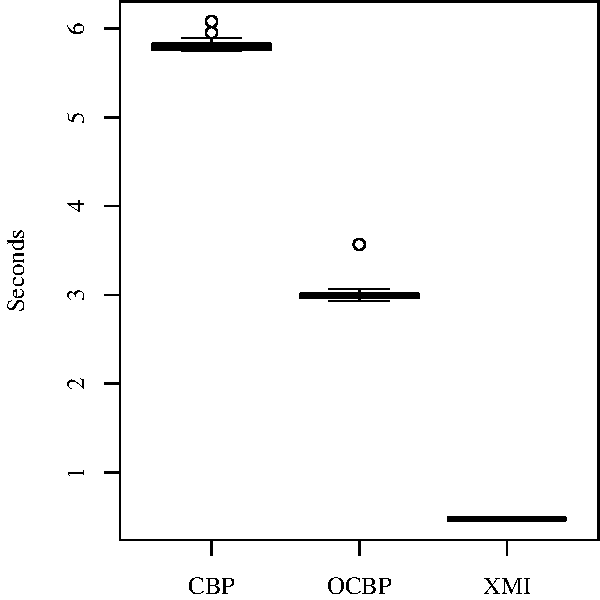
\includegraphics[width=\linewidth]{images/ol_load_time_bpmn2}
\caption{BPMN2}
\label{fig:load_time_bpmn2}
\end{subfigure}
\hfill
\begin{subfigure}{0.325\textwidth}
\centering
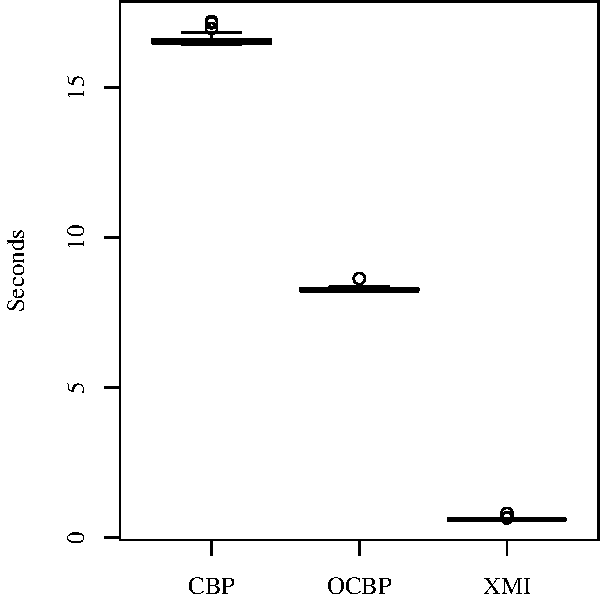
\includegraphics[width=\linewidth]{images/ol_load_time_epsilon}
\caption{Epsilon}
\label{fig:load_time_epsilon}
\end{subfigure}
\hfill
\begin{subfigure}{0.325\textwidth}
\centering
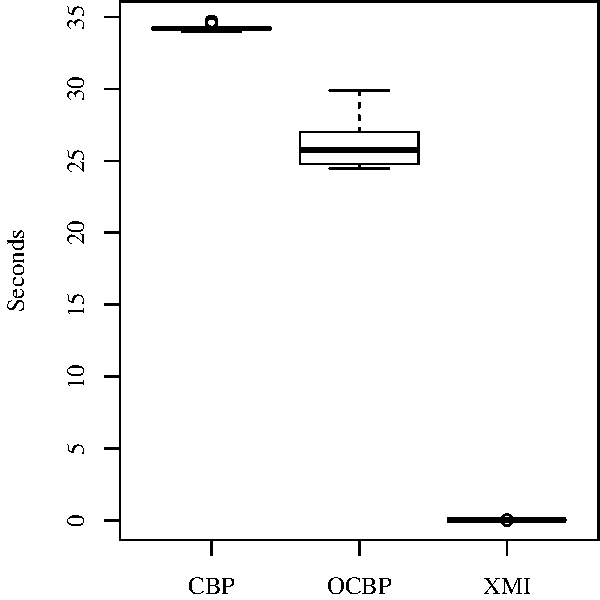
\includegraphics[width=\linewidth]{images/ol_load_time_wikipedia}
\caption{Wikipedia}
\label{fig:load_time_wikipedia}
\end{subfigure}
\caption{Results for loading a model in original CBP (CBP), optimised CBP (OCBP), and for loading a state-based (XMI) representation.}
\label{fig:loadtime}
\end{figure}

\vspace{-25pt}
\subsection{Model Saving Time}
\label{subsec:saving_time_test}

\vspace{-10pt}
This subsection presents the results of the saving time measurement of change-based models for each pair of the persistence types and cases, and the t-test results of their comparisons (Table \ref{table:ttest_results_savetime} and Fig. \ref{fig:savetime}). As discussed in\,\cite{yohannis2017turning}, CBP loading time penalties are balanced against the benefits that CBP brings, in terms of  persisting changes (saving time).

\vspace{-25pt}
\begin{table}[ht]
\footnotesize
\centering
\caption{The t-test results of saving time comparison between original CBP (CBP), optimised CBP (OCBP), and XMI.}
\label{table:ttest_results_savetime}
\begin{tabular}
{|p{0.12\textwidth}p{0.11\textwidth}p{0.13\textwidth}|p{0.22\textwidth}p{0.14\textwidth}p{0.12\textwidth}p{0.10\textwidth}|}
\hline 

% BPMN2 Save Time
Group & Mean & SD & Comparison & t  & df & p-value \\
\hline 
\multicolumn{3}{|c|}{\textbf{BPMN2 Save Time ($s$)}} & \multicolumn{4}{c|}{\textbf{BPMN2 Save Time}}\\
CBP & 0.00097    & 123e-5 & CBP vs. XMI &  -175.58    & 22.01 & $<$ 0.05 \\  
OCBP & 0.00081   & 12e-5 & CBP vs. OCBP & 0.62 & 21.38  & 0.54 \\  
XMI & 0.30122   & 793e-5 & OCBP vs. XMI & -177.76    & 21.01  & $<$ 0.05 \\ 
\hline 

% EPSILON Save Time
\multicolumn{3}{|c|}{\textbf{Epsilon Save Time ($s$)}} & \multicolumn{4}{c|}{\textbf{Epsilon Save Time}}\\
CBP & 0.00069    & 3.4e-5 &  CBP vs. XMI & -6.01   &21.00 & $<$ 0.05 \\
OCBP & 0.00080   & 8.0e-5 & CBP vs. OCBP & 160.06 & 28.24 & $<$ 0.05 \\  
XMI & 0.40025   & 595e-5 & OCBP vs. XMI & -314.80  & 21.01  & $<$ 0.05 \\ 
\hline 

% WIKIPEDIA Save Time
\multicolumn{3}{|c|}{\textbf{Wiki Save Time ($s$)}} & \multicolumn{4}{c|}{\textbf{Wikipedia Save Time}}\\
CBP & 0.00071     & 4.9e-5 & CBP vs. XMI &  -46.19   & 21.08 & $<$ 0.05 \\ 
OCBP &0.00075   &  4.1e-5 & CBP vs. OCBP &   -3.48 & 40.77 & $<$ 0.05 \\ 
XMI &  0.01195   & 114e-5 & OCBP vs. XMI &  -46.01  & 21.06 & $<$ 0.05 \\ 
\hline
\end{tabular}
\justify
$Mean$ = average, $SD$ = standard deviation, $t$ = t-test's $t$-$value$, $df$ = degree of freedom, $p$-$value$ = significance, $s$ = the unit is seconds
\end{table}



As shown in Table \ref{table:ttest_results_savetime} and Fig. \ref{fig:savetime}, the performance of the two CBP implementations is not very different. Since the significance level is 5\%, only the BPMN2 case that fails. However, the difference between the $means$ of its original CBP (0.97 ms) and optimised CBP (0.81 ms) is small. This indicates that the cost of the extra work in the optimised CBP algorithm is negligible. On the other hand, both CBP implementations are significantly faster at saving changes than state-based XMI (the $means$ of both CBP implementations are smaller than XMI's $means$, and both CBP implementations have $p$-$values$ $<$ 0.05 when compared to XMI). This is expected, as the CBP implementations only need append the last changes to the existing model file (their performance is thus relative to the number of changes since the last save), while the XMI implementation needs to reconstruct an XML document for the entire state of the model, and replaces the contents of the model file every time (and hence its performance is relative to the size of the entire model). 

\begin{figure}[t]
\begin{subfigure}{0.325\textwidth}
\centering
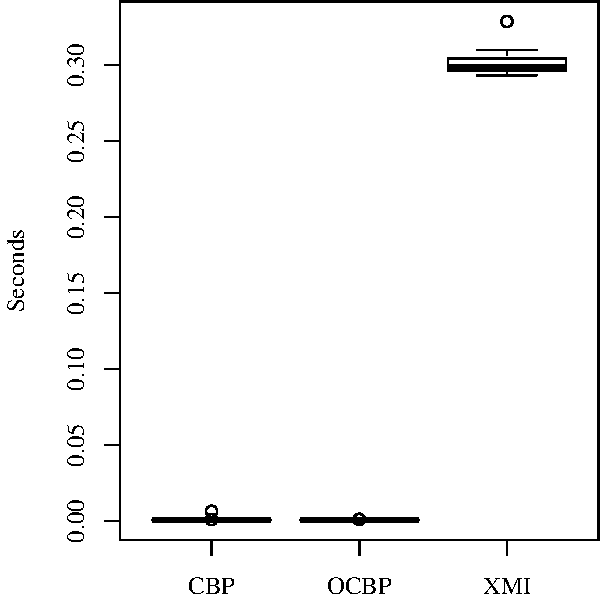
\includegraphics[width=\linewidth]{images/ol_save_time_bpmn2}
\caption{BPMN2}
\label{fig:save_time_bpmn2}
\end{subfigure}
\hfill
\begin{subfigure}{0.325\textwidth}
\centering
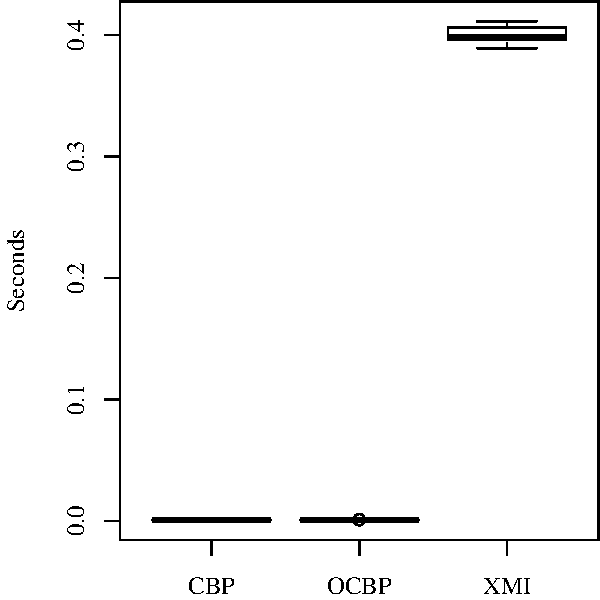
\includegraphics[width=\linewidth]{images/ol_save_time_epsilon}
\caption{Epsilon}
\label{fig:save_time_epsilon}
\end{subfigure}
\hfill
\begin{subfigure}{0.325\textwidth}
\centering
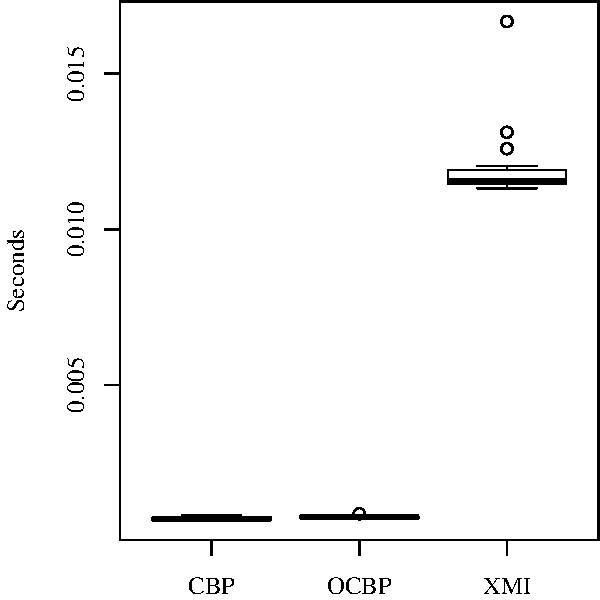
\includegraphics[width=\linewidth]{images/ol_save_time_wikipedia}
\caption{Wikipedia}
\label{fig:save_time_wikipedia}
\end{subfigure}
\caption{A comparison on time required for persisting an event between original CBP (CBP), optimised CBP (OCBP), and XMI.}
\label{fig:savetime}
\end{figure}


\vspace{-10pt}
\subsection{Memory Footprint}
\label{subsec:memory_consumption}


\begin{figure}[ht]
\begin{subfigure}{0.325\textwidth}
\centering
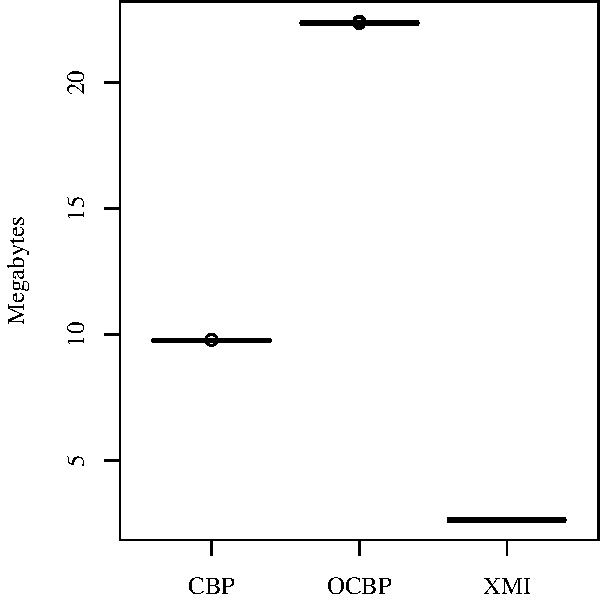
\includegraphics[width=\linewidth]{images/ol_load_memory_bpmn2}
\caption{BPMN2}
\label{fig:load_memory_bpmn2}
\end{subfigure}
\hfill
\begin{subfigure}{0.325\textwidth}
\centering
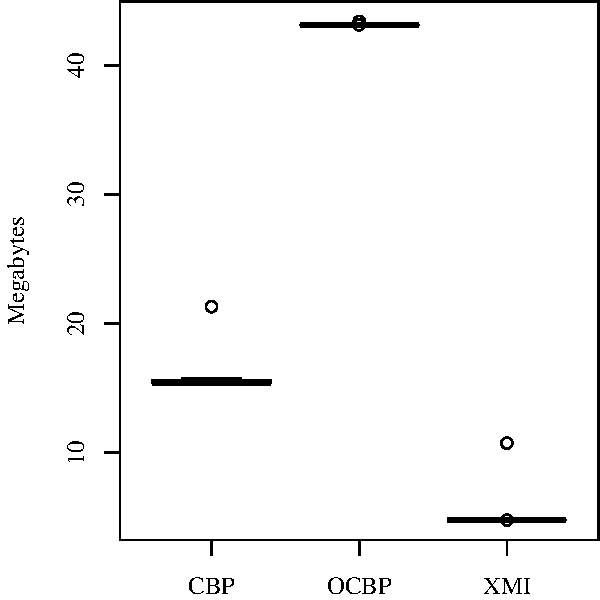
\includegraphics[width=\linewidth]{images/ol_load_memory_epsilon}
\caption{Epsilon}
\label{fig:load_memory_epsilon}
\end{subfigure}
\hfill
\begin{subfigure}{0.325\textwidth}
\centering
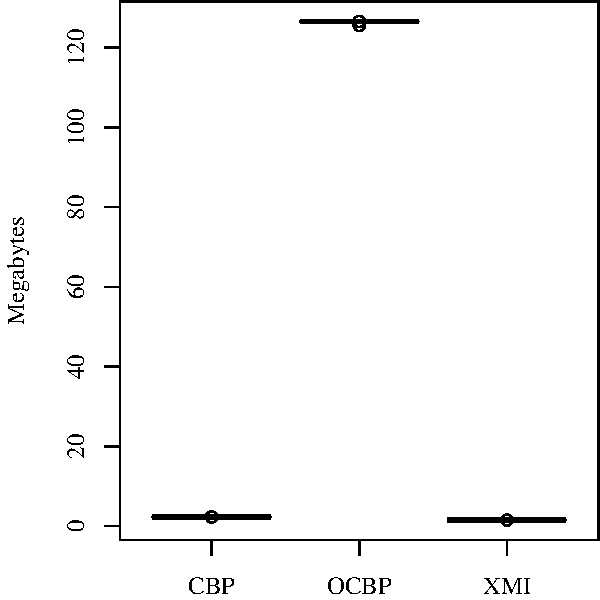
\includegraphics[width=\linewidth]{images/ol_load_memory_wikipedia}
\caption{Wikipedia}
\label{fig:load_memory_wikipedia}
\end{subfigure}
\caption{A comparison on memory footprint after loading a model between original CBP (CBP), optimised CBP (OCBP), and XMI.}
\label{fig:loadmemory}
\end{figure}

\begin{table}[t]
\footnotesize
\centering
\caption{The t-test results of memory footprint comparison after loading a model between original CBP (CBP), optimised CBP (OCBP), and XMI.}
\label{table:ttest_results_load_memory}
\begin{tabular}
{|p{0.12\textwidth}p{0.11\textwidth}p{0.13\textwidth}|p{0.22\textwidth}p{0.14\textwidth}p{0.12\textwidth}p{0.10\textwidth}|}
\hline 

% BPMN2 Load Memory
Group & Mean & SD & Comparison & t  & df & p-value \\
\hline 
\multicolumn{3}{|c|}{\textbf{BPMN2 Load Memory ($M$)}} & \multicolumn{4}{c|}{\textbf{BPMN2 Load Memory}} \\
CBP & 9.76     & 76.0e-4 & CBP vs. XMI &  4,392.5   & 21.22 & $<$ 0.05 \\  
OCBP & 22.36   & 0.015 & CBP vs. OCBP & -3,695.7 & 32.28  & $<$ 0.05 \\  
XMI &  2.63   & 5.5e-4 & OCBP vs. XMI &  6,572.4    & 21.06  & $<$ 0.05 \\ 
\hline 

% EPSILON Load Memory
\multicolumn{3}{|c|}{\textbf{Epsilon Load Memory ($M$)}} & \multicolumn{4}{c|}{\textbf{Epsilon Load Memory}} \\
CBP &15.74    & 1.248 &  CBP vs. XMI & 28.16   &  41.99 & $<$ 0.05 \\
OCBP & 43.15   & 0.056 & CBP vs. OCBP & -102.9 &21.08 & $<$ 0.05 \\  
XMI & 5.05   & 1.271 & OCBP vs. XMI & 140.49  & 21.08  & $<$ 0.05 \\ 
\hline 

% WIKIPEDIA Load Memory
\multicolumn{3}{|c|}{\textbf{Wiki Load Memory ($M$)}} & \multicolumn{4}{c|}{\textbf{Wikipedia Load Memory}} \\
CBP & 2.29  & 2.4e-4 & CBP vs. XMI &   4,523.5   & 25.16 & $<$ 0.05 \\ 
OCBP & 126.48 & 0.29 & CBP vs. OCBP &   -2,009.3 & 21.00 & $<$ 0.05 \\ 
XMI &  1.52  & 7.6e-4 & OCBP vs. XMI &  2,021.8  & 21.00 & $<$ 0.05 \\ 
\hline
\end{tabular}
\justify
$Mean$ = average, $SD$ = standard deviation, $t$ = t-test's $t$-$value$, $df$ = degree of freedom, $p$-$value$ = significance, $M$ = the unit is megabytes
\end{table}

\vspace{-10pt}
\begin{figure}
\begin{subfigure}{0.325\textwidth}
\centering
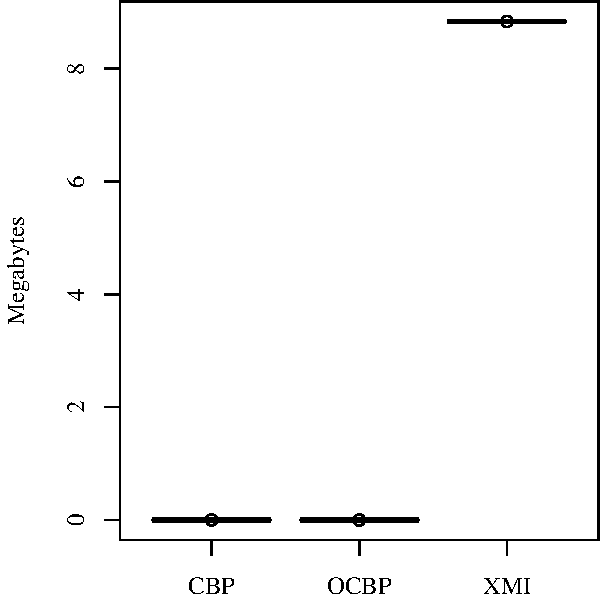
\includegraphics[width=\linewidth]{images/ol_save_memory_bpmn2}
\caption{BPMN2}
\label{fig:save_memory_bpmn2}
\end{subfigure}
\hfill
\begin{subfigure}{0.325\textwidth}
\centering
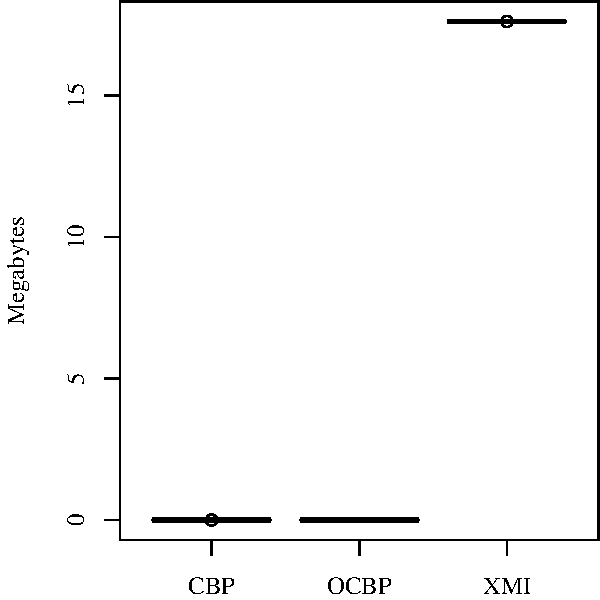
\includegraphics[width=\linewidth]{images/ol_save_memory_epsilon}
\caption{Epsilon}
\label{fig:save_memory_epsilon}
\end{subfigure}
\hfill
\begin{subfigure}{0.325\textwidth}
\centering
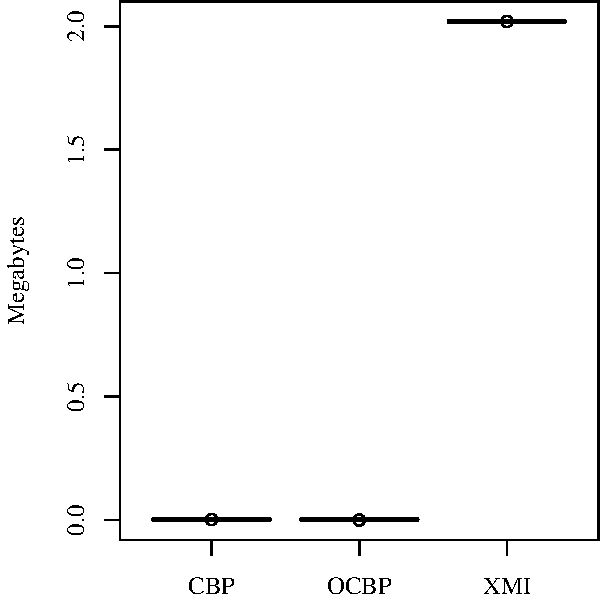
\includegraphics[width=\linewidth]{images/ol_save_memory_wikipedia}
\caption{Wikipedia}
\label{fig:save_memory_wikipedia}
\end{subfigure}
\caption{A comparison on memory footprint after persisting an event between CBP, optimised CBP, and XMI.}
\label{fig:savememory}
\end{figure}

\begin{table}[t]
\footnotesize
\centering
\caption{The t-test results of memory footprint comparison after saving an event between original CBP (CBP), optimised CBP (OCBP), and XMI.}
\label{table:ttest_results_save_memory}
\begin{tabular}
{|p{0.12\textwidth}p{0.11\textwidth}p{0.13\textwidth}|p{0.22\textwidth}p{0.14\textwidth}p{0.12\textwidth}p{0.10\textwidth}|}
\hline 

% BPMN2 Save Memory
Group & Mean & SD & Comparison & t  & df & p-value \\
\hline 
\multicolumn{3}{|c|}{\textbf{BPMN2 Save Memory ($M$)}} & \multicolumn{4}{c|}{\textbf{BPMN2 Save Memory}} \\
CBP &0.0023    & 6.3e-5 & CBP vs. XMI &  -489,170    & 41.49 & $<$ 0.05 \\  
OCBP &0.0029    & 80e-5 & CBP vs. OCBP & -3.22 & 21.26 & $<$ 0.05 \\
XMI & 8.84   & 5.6e-5 & OCBP vs. XMI & -51,180    &  21.21  & $<$ 0.05 \\ 
\hline 

% EPSILON Save Memory
\multicolumn{3}{|c|}{\textbf{Epsilon Save Memory ($M$)}} & \multicolumn{4}{c|}{\textbf{Epsilon Save Memory}}\\
CBP & 0.0025    & 18.8e-6 &  CBP vs. XMI & -4.3e\texttt{+}6   & 21.00 & $<$ 0.05 \\
OCBP & 0.0031    & 279.9e-6 & CBP vs. OCBP & -10.131 & 21.19 & $<$ 0.05 \\ %1.41e-09 \\  
XMI & 17.61   & 2.4e-6 & OCBP vs. XMI & -295,090  &21.00  & $<$ 0.05 \\ 
\hline 

% WIKIPEDIA Save Memory
\multicolumn{3}{|c|}{\textbf{Wiki Save Memory ($M$)}} & \multicolumn{4}{c|}{\textbf{Wikipedia Save Memory}} \\
CBP & 0.0025  &1.9e-5 & CBP vs. XMI &  -391,970   & 40.52 & $<$ 0.05 \\ 
OCBP &  0.0028   & 84.1e-5 & CBP vs. OCBP &  -1.75 & 21.02 &  0.094 \\ 
XMI &  2.0194   & 1.5e-5 & OCBP vs. XMI &  -11,245  & 21.01 & $<$ 0.05 \\ 
\hline
\end{tabular}
\justify
$Mean$ = average, $SD$ = standard deviation, $t$ = t-test's $t$-$value$, $df$ = degree of freedom, $p$-$value$ = significance, $M$ = the unit is megabytes
\end{table}

Here we present the results of measuring the memory footprint after loading models (Table \ref{table:ttest_results_load_memory} and Fig. \ref{fig:loadmemory}) and persisting single changes (Table \ref{table:ttest_results_save_memory} and Fig. \ref{fig:savememory}) using the models from the three cases. The results show the significant memory overhead of the extra data structure when loading models (all the $means$ of optimised CBP are greater than all the $means$ of original CBP and all comparisons between both CBPs show $p$-$values$ $<$ 0.05, Table \ref{table:ttest_results_load_memory}). Both CBPs are also outperformed by XMI in terms of memory footprint when loading models (all the $means$ of XMI are smaller than all the $means$ of both CBPs and all comparisons against XMIs show all $p$-$values$ $<$ 0.05, Table \ref{table:ttest_results_load_memory}). In loading, XMI uses significantly less memory than the optimised CBP representation and performs slightly better than the original CBP.   

In terms of saving, both CBP implementations persist a single change faster than XMI indicated by their $means$ that are smaller than the $means$ of XMI, and all the CBPs' t-tests with XMI show that their differences are significant at $p$-$value$ $<$ 0.05 (Table \ref{table:ttest_results_save_memory}). The optimised CBP has a larger memory footprint than the original CBP since the means of the optimised CBP for all cases are greater than the means of the original CBP. However, their memory footprints are not very different. Even though the BPMN2 and Epsilon cases have $p$-$values$ $<$ 0.05, the differences of the $means$ of their original and optimised CBPs are small, and the Wikipedia case also shows $p$-$value$ $>$ 0.05 on its original CBP vs. optimised CBP comparison.   

\vspace{-15pt}
\subsection{Threats to Validity and Limitations}
\label{sec:limitations_and_future_work}

\vspace{-10pt}
In this work, we have only tested the algorithms on synthesised  models which may not be representative of the complexity and interconnectedness of models in other domains. Diverse characteristics of models in different domains can affect the effectiveness of the algorithm and therefore yield different outcomes. So far, CBP optimisation only supports ordered and unique features. Support for duplicate values means that removal of an item does not necessarily result in the item not being present in the feature value. Additional information must be captured to persist the number of copies and positions of the feature members to properly generate the ignore list. 

\vspace{-15pt}
\subsection{Discussion}
\label{sec:discussion}

\vspace{-10pt}
For the original CBP loading, the total time required to load a model is $T_{CBP}$ = $T_E$ + $T_O$, where $T_E$ is the total time required to complete executing all events, and $T_O$ is the total time needed to complete other required routines (e.g. initialisation, reading files). For the optimised CBP loading, the total time to load a change-based model is reduced by the total time saved-up by ignoring superseded events $T_I$, that is $T_{OCBP}$ = $T_E$ + $T_O$ $-$ $T_I$. Thus, it is expected that optimised CBP can load a model faster than original CBP. This statement is in accordance with our finding in Section \ref{subsec:loading_time_test} that the total saved-up loading time corresponds to the number of ignored events. However, it still requires more investigation to determine the degree of their correlation, which will be addressed in our future work.

\vspace{-5pt}
\section{Conclusions and Future Work}
\label{sec:conclusions}
This paper proposes an efficient algorithm and supporting data structures for loading change-based models.  Performance is evaluated on synthesised models, with comparison against the existing change-based implementation, and state-based XMI. Our results show considerable savings in terms of loading time with a negligible impact on saving time, but at the cost of a higher memory footprint.  In future, we intend to evaluate CBP against state-based persistence on real complex models.  We also plan to investigate the impact of change-based model persistence on the performance of change detection, model merging, and conflict resolution in the context of collaborative modelling. Meanwhile, the CBP approach can be further optimised to consume less memory and speed up parsing, such as using binary format instead of text. We are also exploring a hybrid persistence representation that offers a combination of state-based and change-based persistence. 


